\documentclass[UTF8,zihao=-4,fontset=windows]{ctexart}

\usepackage[a4paper,margin=2.25cm,headheight=15pt]{geometry}
\usepackage{graphicx}
\usepackage{booktabs}
\usepackage{tabularx}
\usepackage{array}
\usepackage{enumitem}
\usepackage{xcolor}
\usepackage{fancyhdr}
\usepackage{titlesec}
\usepackage{caption}
\usepackage{hyperref}
\usepackage{float}
\usepackage{amsmath}
\usepackage{listings}

\definecolor{navy}{HTML}{000000}
\definecolor{teal}{HTML}{000000}
\definecolor{pale}{HTML}{F3F3F3}
\definecolor{muted}{HTML}{555555}
\definecolor{codebg}{HTML}{F6F6F6}

\hypersetup{colorlinks=true,linkcolor=black,urlcolor=black,citecolor=black,
  pdftitle={自动驾驶技术第一次实验报告},pdfauthor={杜承敖}}
\graphicspath{{assets/}}
\setlength{\parindent}{2em}
\setlength{\parskip}{0.28em}
\setlength{\emergencystretch}{2em}
\renewcommand{\arraystretch}{1.18}
\setcounter{tocdepth}{2}
\captionsetup{font=small,labelfont={bf},skip=6pt}
\setlist[itemize]{leftmargin=2em,itemsep=0.2em,topsep=0.3em}

\lstset{language=Python,basicstyle=\ttfamily\scriptsize,frame=single,
  backgroundcolor=\color{codebg},columns=fullflexible,breaklines=true,
  showstringspaces=false,xleftmargin=0.6em,xrightmargin=0.6em,
  aboveskip=0.45em,belowskip=0.35em}

\titleformat{\section}{\Large\bfseries\color{navy}}{\thesection}{0.7em}{}
\titleformat{\subsection}{\large\bfseries\color{teal}}{\thesubsection}{0.7em}{}
\titlespacing*{\section}{0pt}{1.0em}{0.45em}
\titlespacing*{\subsection}{0pt}{0.7em}{0.3em}

\pagestyle{fancy}
\fancyhf{}
\fancyhead[L]{\small 自动驾驶技术第一次实验}
\fancyhead[R]{\small nuScenes 多传感器数据与 YOLO 检测}
\fancyfoot[C]{\small\color{muted}\thepage}
\renewcommand{\headrulewidth}{0.4pt}

\begin{document}

\begin{titlepage}
  \thispagestyle{empty}
  \begin{center}
    \vspace*{1.8cm}
    {\zihao{1}\bfseries 自动驾驶技术第一次实验报告\par}
    \vspace{1.0cm}
    {\zihao{3}\bfseries nuScenes Boston Seaport\par}
    \vspace{0.25cm}
    {\zihao{3}\bfseries 多传感器数据与 YOLO 目标检测\par}

    \vfill

    {\zihao{4}
    \renewcommand{\arraystretch}{1.75}
    \begin{tabular}{>{\bfseries}r l}
      姓名： & \underline{\makebox[9.2cm][c]{杜承敖}} \\
      学号： & \underline{\makebox[9.2cm][c]{2024302112019}} \\
      专业： & \underline{\makebox[9.2cm][c]{计算机科学与技术（雷军班）}} \\
      课程： & \underline{\makebox[9.2cm][c]{自动驾驶技术}} \\
    \end{tabular}
    }

    \vfill

    {\zihao{3}\bfseries 武汉大学\par}
    \vspace{0.45cm}
    {\zihao{4}2026 年 9 月 28 日\par}
    \vspace*{0.8cm}
  \end{center}
\end{titlepage}

\pagenumbering{arabic}

\tableofcontents
\clearpage

\phantomsection
\section*{摘要}
\addcontentsline{toc}{section}{摘要}

本报告记录一次以 nuScenes Boston Seaport 为对象的多传感器数据实践。首先使用官方 devkit 读取场景、关键帧、标定和位姿表，核对原始数据与 YOLO 数据集的组织关系；随后将全局坐标系中的 3D 标注框和 LiDAR 点云变换到相机坐标系并投影到 CAM\_FRONT 图像。实测样本来自 scene-0161，包含 34,720 个 LiDAR 原始点，其中 2,769 个点投影到相机可见区域，10 个完整可见的 3D 标注框被投影为图像线框。最后，使用转换后的 10 类二维检测数据训练 YOLO11n 20 轮，并以独立 test 集给出最终结果：Precision 0.511、Recall 0.394、mAP50 0.403、mAP50--95 0.217。报告明确区分实际生成的图表、可复现代码和本地数据包的限制。

\noindent\textbf{关键词：}nuScenes；Boston Seaport；多传感器融合；坐标投影；YOLO11n

\clearpage

\section{实验任务与完成链路}

本次实验不从训练结果直接开始，而是沿着“原始数据---坐标与标注---二维检测数据---模型评估”的链路记录工作。这样做的原因是：YOLO 的二维框来自 nuScenes 的三维标注和相机标定；若不说明数据组织和坐标变换，训练指标就无法对应到原始传感器数据。

完成的工作分为四部分：
\begin{itemize}
  \item 读取 v1.0-trainval 的 JSON 元数据，统计四种采集地点的场景，并访问一个 Boston Seaport 关键帧的全部传感器记录；
  \item 核对原始目录、表之间的 token 关系，以及转换后 YOLO 图像、标签、数据拆分和类别编号；
  \item 用 devkit 的标定、位姿、3D Box 和点云对象完成 3D 标注框到 2D 图像的投影，以及 LiDAR 到 CAM\_FRONT 的叠加显示；
  \item 在转换后的 Boston Seaport 数据上训练 YOLO11n 20 轮，使用验证集选择权重，在独立 test 集上完成一次评估和预测可视化。
\end{itemize}

这份报告中的 devkit 图由 \texttt{scripts/build\_devkit\_evidence.py} 实际运行生成；YOLO 曲线、混淆矩阵和预测图来自 \texttt{yolo\_workflow} 的正式运行目录。

\section{数据集格式与组织}

\subsection{原始 nuScenes 数据表与目录}

nuScenes 不把一次采集简单存为“图片加标签”。每条记录由 token 连接：\texttt{scene} 描述一段驾驶片段，\texttt{sample} 表示一个关键帧，\texttt{sample\_data} 指向各传感器文件，\texttt{calibrated\_sensor} 和 \texttt{ego\_pose} 给出坐标变换。三维标注位于 \texttt{sample\_annotation}，其中包含类别、中心、尺寸、朝向、实例和可见度等信息。

\begin{table}[H]
  \centering
  \caption{本次使用的原始数据组织与作用}
  \begin{tabularx}{\textwidth}{>{\raggedright\ttfamily\scriptsize\arraybackslash}p{3.6cm}X}
    \toprule
    位置或表 & 实验中的作用 \\
    \midrule
    scene.json & 场景名称、首末关键帧和 log 的连接 \\
    sample.json & 一个关键帧的 12 路传感器 token 与标注 token \\
    sample\_data.json & 传感器文件名、时间戳、标定和位姿 token \\
    calibrated\_sensor.json / ego\_pose.json & 传感器外参、相机内参和车辆在全局坐标系中的位姿 \\
    sample\_annotation.json & 全局坐标系中的 3D 标注框及其类别和实例关系 \\
    CAM\_FRONT / LIDAR\_TOP & 本地课程包中可用的前视图像和顶置 LiDAR 原始文件 \\
    \bottomrule
  \end{tabularx}
\end{table}

元数据覆盖 850 个场景、34,149 个关键帧。按照 \texttt{log.location} 统计，地点构成如表\ref{tab:location}。本报告的训练部分只使用 Boston Seaport；其他地点的场景仍通过同一套 devkit 表结构访问。

\begin{table}[H]
  \centering
  \caption{v1.0-trainval 场景地点统计}
  \label{tab:location}
  \begin{tabular}{lr}
    \toprule
    采集地点 & 场景数 \\
    \midrule
    boston-seaport & 467 \\
    singapore-onenorth & 183 \\
    singapore-queenstown & 115 \\
    singapore-hollandvillage & 85 \\
    \midrule
    合计 & 850 \\
    \bottomrule
  \end{tabular}
\end{table}

\subsection{转换后的 YOLO 数据集}

为训练二维检测器，原始三维标注被转换为相机图像上的二维矩形框，并写成 YOLO 标签行：
\[
\texttt{class\_id\ \ c\_x\ \ c\_y\ \ w\ \ h},
\]
其中 $c_x,c_y,w,h$ 都按图像宽高归一化。Boston Seaport 转换结果保留 10 类：car、truck、bus、trailer、construction\_vehicle、pedestrian、motorcycle、bicycle、traffic\_cone、barrier。类别顺序存放于 \texttt{data.yaml} 和 \texttt{classes.txt}，训练、验证和测试使用同一映射。

\begin{table}[H]
  \centering
  \caption{转换后 YOLO 数据集的目录和拆分}
  \begin{tabularx}{\textwidth}{>{\ttfamily\small}p{5.2cm}Xr}
    \toprule
    目录或文件 & 内容 & 帧数 \\
    \midrule
    \textnormal{images/train, labels/train} & 训练图像及对应 YOLO 文本标签 & 9,420 \\
    \textnormal{images/val, labels/val} & 每轮训练后的验证数据 & 1,402 \\
    \textnormal{images/test, labels/test} & 最终独立评估数据 & 2,709 \\
    \textnormal{data.yaml, classes.txt} & 路径、拆分和 10 类映射 & -- \\
    \textnormal{manifest.csv 与转换摘要} & 转换与拆分记录，随机种子为 42 & -- \\
    \bottomrule
  \end{tabularx}
\end{table}

转换摘要的实际文件名为 \texttt{conversion\_summary.json}。三种拆分共 13,531 帧，约为 7:1:2。训练过程只访问 train 和 val；test 保留到模型选择完成后，因此它的数值不用于调参。

\section{nuScenes devkit 的场景与传感器使用}

\subsection{场景、关键帧和传感器调用}

devkit 的访问以 \texttt{NuScenes} 对象为入口。代码清单\ref{lst:devkit}先通过 \texttt{log.location} 枚举所有地点场景，再找到一个 Boston Seaport 场景，并从首个关键帧的 \texttt{data} 字段依次读取各个传感器。循环方式比手动写 12 次调用更可靠：它直接使用 sample 中实际存在的 channel 和 token。

\begin{lstlisting}[caption={使用 devkit 访问场景、关键帧和全部传感器},label={lst:devkit}]
from nuscenes.nuscenes import NuScenes

nusc = NuScenes(version="v1.0-trainval", dataroot="nuscenes",
                verbose=False)
locations = {
    nusc.get("log", scene["log_token"])["location"]
    for scene in nusc.scene
}
scene = next(
    s for s in nusc.scene
    if nusc.get("log", s["log_token"])["location"] == "boston-seaport"
)
sample = nusc.get("sample", scene["first_sample_token"])
for channel, token in sorted(sample["data"].items()):
    sample_data = nusc.get("sample_data", token)
    calibrated = nusc.get(
        "calibrated_sensor", sample_data["calibrated_sensor_token"]
    )
    sensor = nusc.get("sensor", calibrated["sensor_token"])
    print(channel, sensor["modality"], sample_data["filename"])
\end{lstlisting}

实际运行时选中的样本为 \texttt{scene-0161}，地点为 Boston Seaport。该 keyframe 的传感器清单见表\ref{tab:sensor}。CAM\_FRONT 和 LIDAR\_TOP 的原始文件在课程包中可用，其他五路相机和五路 Radar 的元数据可正常读取，但对应二进制文件没有随本地课程包提供。

\begin{table}[H]
  \centering
  \caption{scene-0161 一个关键帧的 12 路传感器记录}
  \label{tab:sensor}
  \begin{tabularx}{0.92\textwidth}{>{\ttfamily\small}p{4.4cm}>{\ttfamily\small}p{1.5cm}X}
    \toprule
    通道 & 模态 & 本地原始文件 \\
    \midrule
    CAM\_FRONT, CAM\_BACK, CAM\_FRONT\_LEFT & camera & 仅 CAM\_FRONT 可用 \\
    CAM\_FRONT\_RIGHT, CAM\_BACK\_LEFT, CAM\_BACK\_RIGHT & camera & 未提供 \\
    LIDAR\_TOP & lidar & 可用 \\
    RADAR\_FRONT, RADAR\_FRONT\_LEFT, RADAR\_FRONT\_RIGHT & radar & 未提供 \\
    RADAR\_BACK\_LEFT, RADAR\_BACK\_RIGHT & radar & 未提供 \\
    \bottomrule
  \end{tabularx}
\end{table}

\subsection{传感器数据显示与可用数据检查}

对可用的 LIDAR\_TOP 文件，devkit 的 \texttt{LidarPointCloud.from\_file} 读取到 34,720 个点。图\ref{fig:lidar-top}以 LiDAR 坐标系显示其俯视分布；红色叉号是自车原点。该图可用于直接检查扫描线、道路边界与近距离车辆是否处于合理位置，也为后续投影提供了原始点坐标。

\begin{figure}[H]
  \centering
  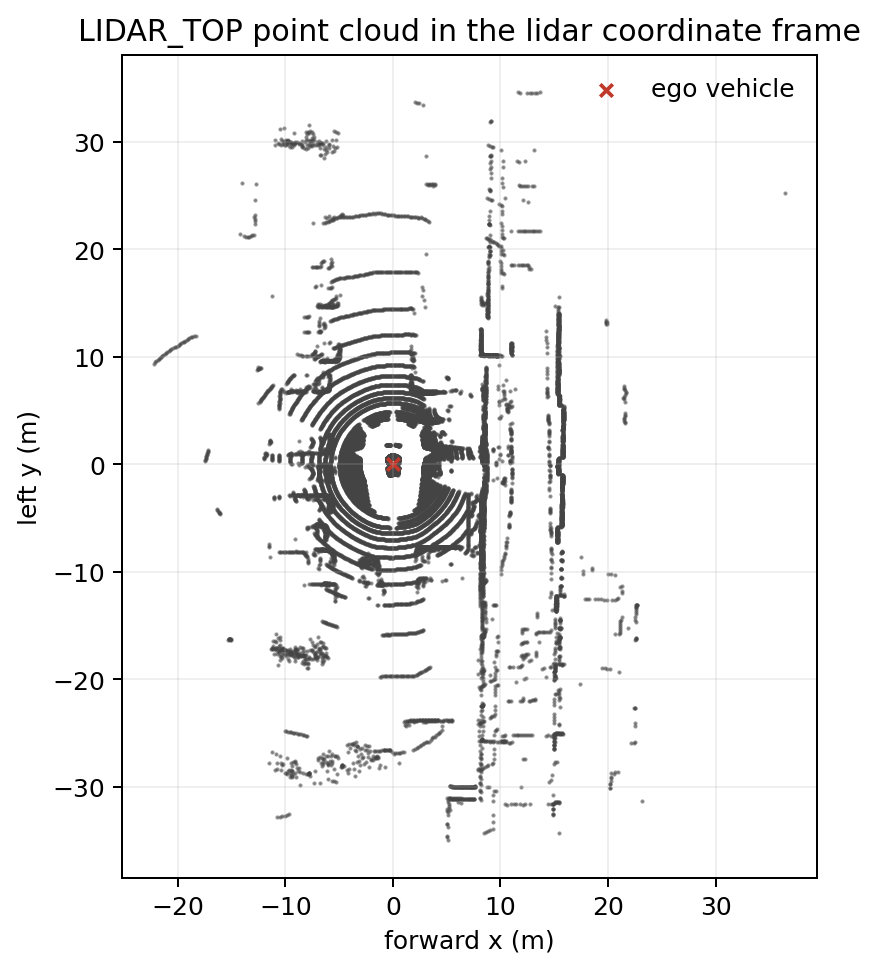
\includegraphics[width=0.66\textwidth]{lidar_topdown.png}
  \caption{scene-0161 同步 LIDAR\_TOP 原始点云的俯视显示。图中保留 $x\in[-25,55]$ m、$y\in[-35,35]$ m 的点。}
  \label{fig:lidar-top}
\end{figure}

Radar 的读取代码使用 \texttt{RadarPointCloud.from\_file}，并与 LiDAR 共用同一投影函数。运行时五个 Radar 路径均被检查为不存在，因此没有把空白图或模拟点写入结果。该限制来自本地数据包，只影响 Radar 的实际显示，不影响 scene、sensor、标定和文件名元数据的调用。

\section{3D 到 2D 的转换与多传感器叠加}

\subsection{统一坐标系与投影步骤}

nuScenes 中的 3D 标注框通常给在全局坐标系，LiDAR 点也首先处于各自传感器坐标系。为了与相机图像叠加，不能只使用相机内参。对一个源传感器点 $p_S$，本实验按“源传感器---源时刻自车---全局---相机时刻自车---相机”的顺序进行变换：
\[
p_C =
T_{C\leftarrow E(t_C)}
T_{E(t_C)\leftarrow G}
T_{G\leftarrow E(t_S)}
T_{E(t_S)\leftarrow S}p_S .
\]
其中各 $T$ 分别由 \texttt{calibrated\_sensor} 和 \texttt{ego\_pose} 的旋转、平移给出。得到相机坐标 $p_C=(x_C,y_C,z_C)$ 后，以相机内参矩阵 $K$ 进行透视投影：
\[
\lambda [u,v,1]^T=Kp_C,\qquad \lambda=z_C.
\]
仅保留 $z_C>0$、落在图像边界内且深度小于 80 m 的点。这样既避免将相机后方点投到图像上，也避免远距稀疏点掩盖近处结构。

\begin{lstlisting}[caption={3D 标注与 LiDAR/Radar 点云到相机平面的核心调用},label={lst:projection}]
from nuscenes.utils.data_classes import LidarPointCloud, RadarPointCloud
from nuscenes.utils.geometry_utils import BoxVisibility, view_points

# 3D annotation box (already expressed in camera coordinates by devkit).
_, boxes, K = nusc.get_sample_data(
    camera_sd["token"], box_vis_level=BoxVisibility.ANY
)
for box in boxes:
    uv = view_points(box.corners(), K, normalize=True)[:2]

# LiDAR and Radar use the same extrinsics/ego-pose projection function.
lidar = LidarPointCloud.from_file(str(lidar_path))
lidar_uv, lidar_depth = project_sensor_to_camera(
    nusc, lidar_sd, camera_sd, lidar.points[:3]
)
radar = RadarPointCloud.from_file(str(radar_path))
radar_uv, radar_depth = project_sensor_to_camera(
    nusc, radar_sd, camera_sd, radar.points[:3]
)
\end{lstlisting}

代码清单\ref{lst:projection}中的 \texttt{project\_sensor\_to\_camera} 在附带脚本中实际实现，并对 LiDAR 运行。Radar 分支保留相同的标定、位姿和投影逻辑；但由于本地没有 \texttt{radar\_path} 所指向的 PCD 文件，不能产生真实 Radar 叠加图。该状态在 \texttt{devkit\_summary.json} 中记录为 \texttt{radar\_overlays\_rendered: 0}。

\subsection{3D 标注框转换为 2D 图像框}

对每个 \texttt{sample\_annotation}，devkit 返回相机坐标系中的 \texttt{Box}。本实验投影其 8 个角点，保留完整落在画面内的框，再以投影点的 $u,v$ 最小值和最大值构成二维外接矩形。图\ref{fig:box}展示了同一帧的实际投影结果：10 个 3D 标注框完整落入图像边界。YOLO 数据转换正是把这类二维矩形映射到类别编号并归一化后写入标签文件。

\begin{figure}[H]
  \centering
  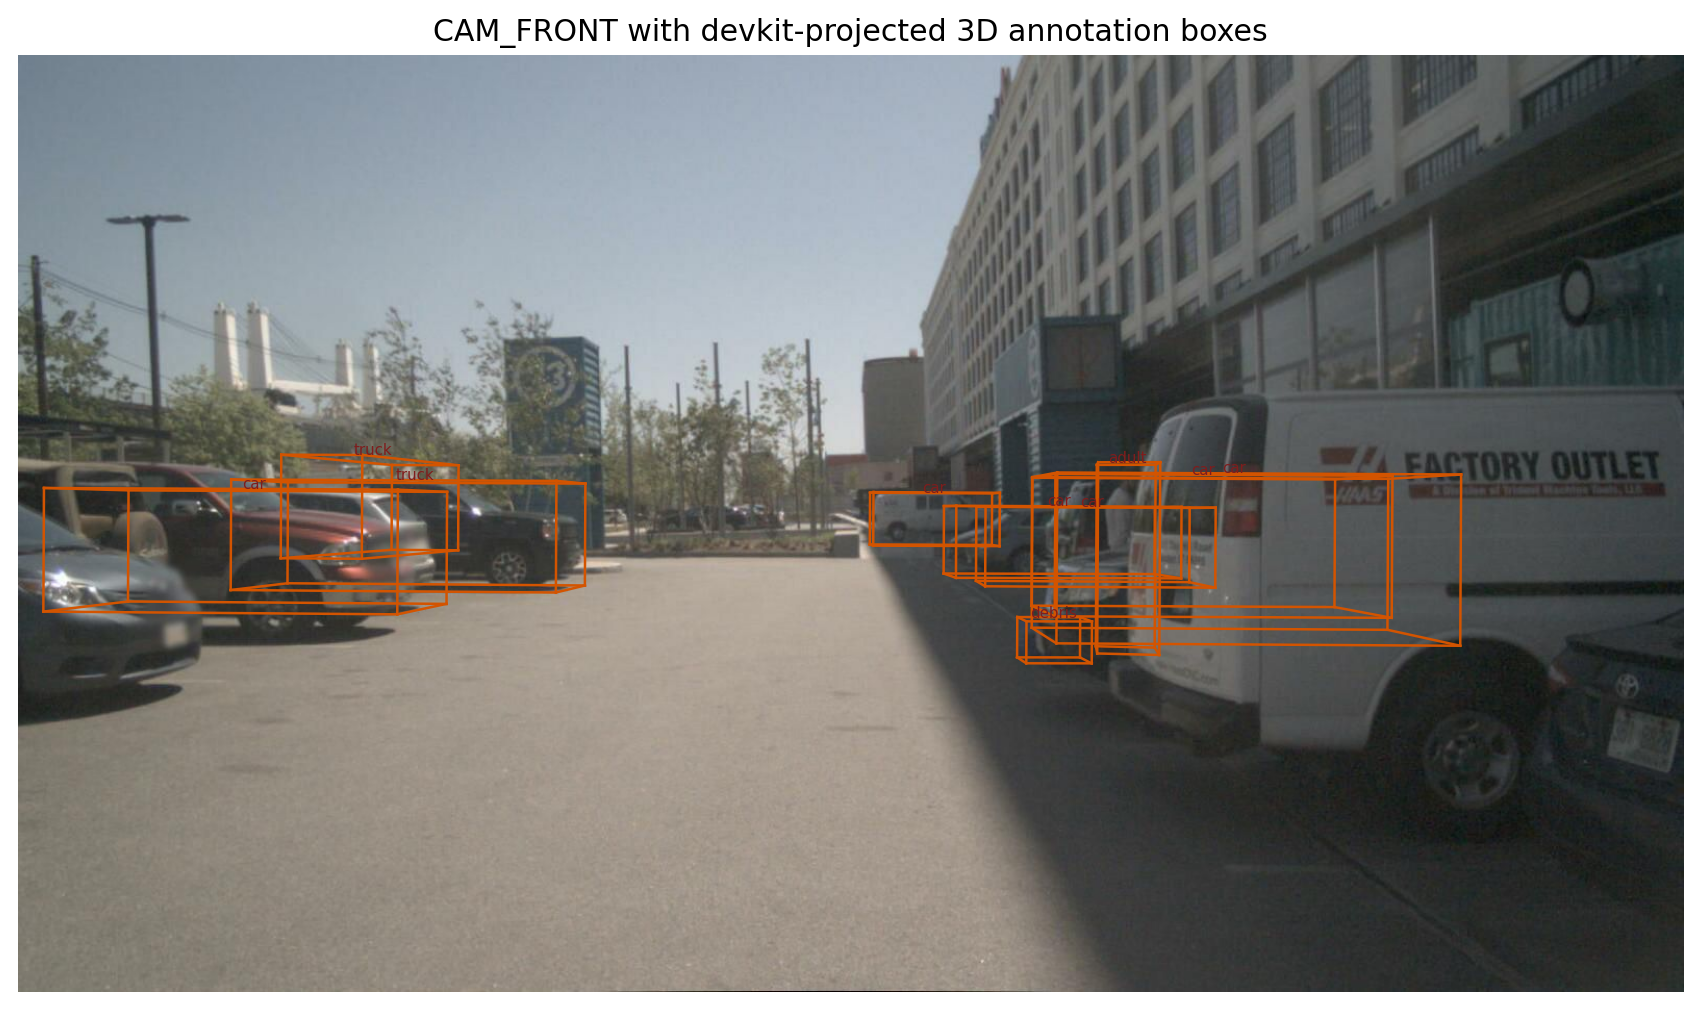
\includegraphics[width=\textwidth]{camera_3d_to_2d_boxes.png}
  \caption{由 devkit 3D Box 角点投影得到的相机图像线框。为便于检查，图中仅显示八个角均位于画面内的 10 个标注框。}
  \label{fig:box}
\end{figure}

\subsection{LiDAR 点云与图像叠加及 Radar 数据限制}

图\ref{fig:lidar-camera}将同一关键帧的 LIDAR\_TOP 点投到 CAM\_FRONT。34,720 个原始点中有 2,769 个同时满足前方、深度和图像边界条件；颜色表示相机坐标系深度。车辆轮廓、路面和建筑立面上的点分布与图像结构相符，说明外参、位姿和内参的组合顺序能够将两种传感器对齐。

\begin{figure}[H]
  \centering
  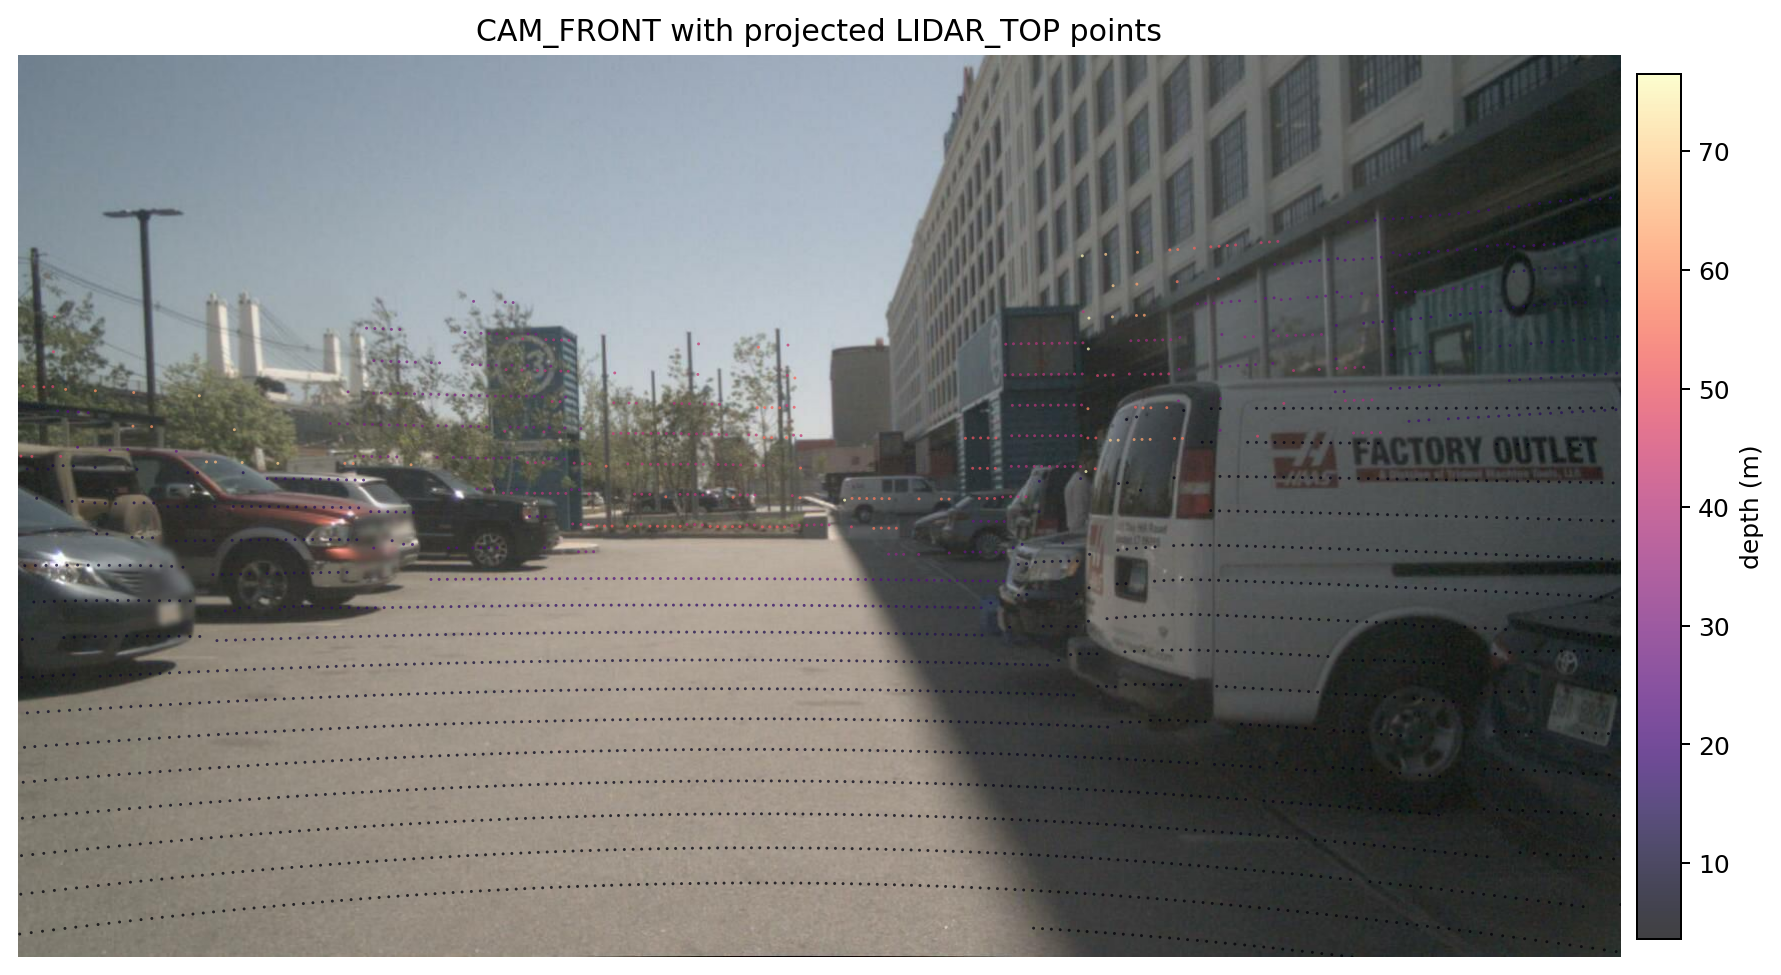
\includegraphics[width=\textwidth]{camera_lidar_overlay.png}
  \caption{CAM\_FRONT 图像与投影后的 LIDAR\_TOP 点云叠加。图中 2,769 个点按照深度着色。}
  \label{fig:lidar-camera}
\end{figure}

Radar 与 LiDAR 的差异在于原始点字段和噪声特性，坐标转换链路相同。由于本地课程包没有 Radar PCD 文件，本报告提供了可运行的 Radar devkit 调用和投影代码，但不把 LiDAR 图误称为 Radar 结果。补齐任一路 Radar 原始文件后，使用同一脚本即可生成对应的 \texttt{camera\_radar\_...\_overlay.png}。

\section{YOLO 训练、日志与独立测试}

\subsection{训练设置与日志}

二维检测训练从预训练 YOLO11n 开始，输入尺寸为 640，batch size 为 8，使用 device 0 和 4 个数据加载线程，共训练 20 epochs。训练结果保存在 \path{yolo_workflow/runs/checkpoints/boston_20ep}；其中 \texttt{args.yaml} 记录参数，\texttt{results.csv} 逐轮保存损失和验证指标，\texttt{best.pt} 与 \texttt{last.pt} 保存模型状态。

图\ref{fig:train}来自训练日志。训练损失持续下降，验证集 mAP50 从第 1 轮的 0.297 升至第 20 轮的 0.443，mAP50--95 从 0.155 升至 0.249。第 15 轮附近指标有小幅波动，属于验证集上的正常变化；模型选择依赖整个验证过程保存的最佳权重，而不是从 test 集挑选结果。

\begin{table}[H]
  \centering
  \caption{训练过程中记录的验证集指标（不是 test 成绩）}
  \begin{tabular}{crrrrr}
    \toprule
    Epoch & Precision & Recall & mAP50 & mAP50--95 & 验证框损失 \\
    \midrule
    1 & 0.667 & 0.274 & 0.297 & 0.155 & 1.615 \\
    5 & 0.580 & 0.349 & 0.388 & 0.208 & 1.532 \\
    10 & 0.595 & 0.417 & 0.433 & 0.241 & 1.492 \\
    15 & 0.522 & 0.418 & 0.425 & 0.235 & 1.497 \\
    20 & 0.632 & 0.414 & 0.443 & 0.249 & 1.480 \\
    \bottomrule
  \end{tabular}
\end{table}

\begin{figure}[H]
  \centering
  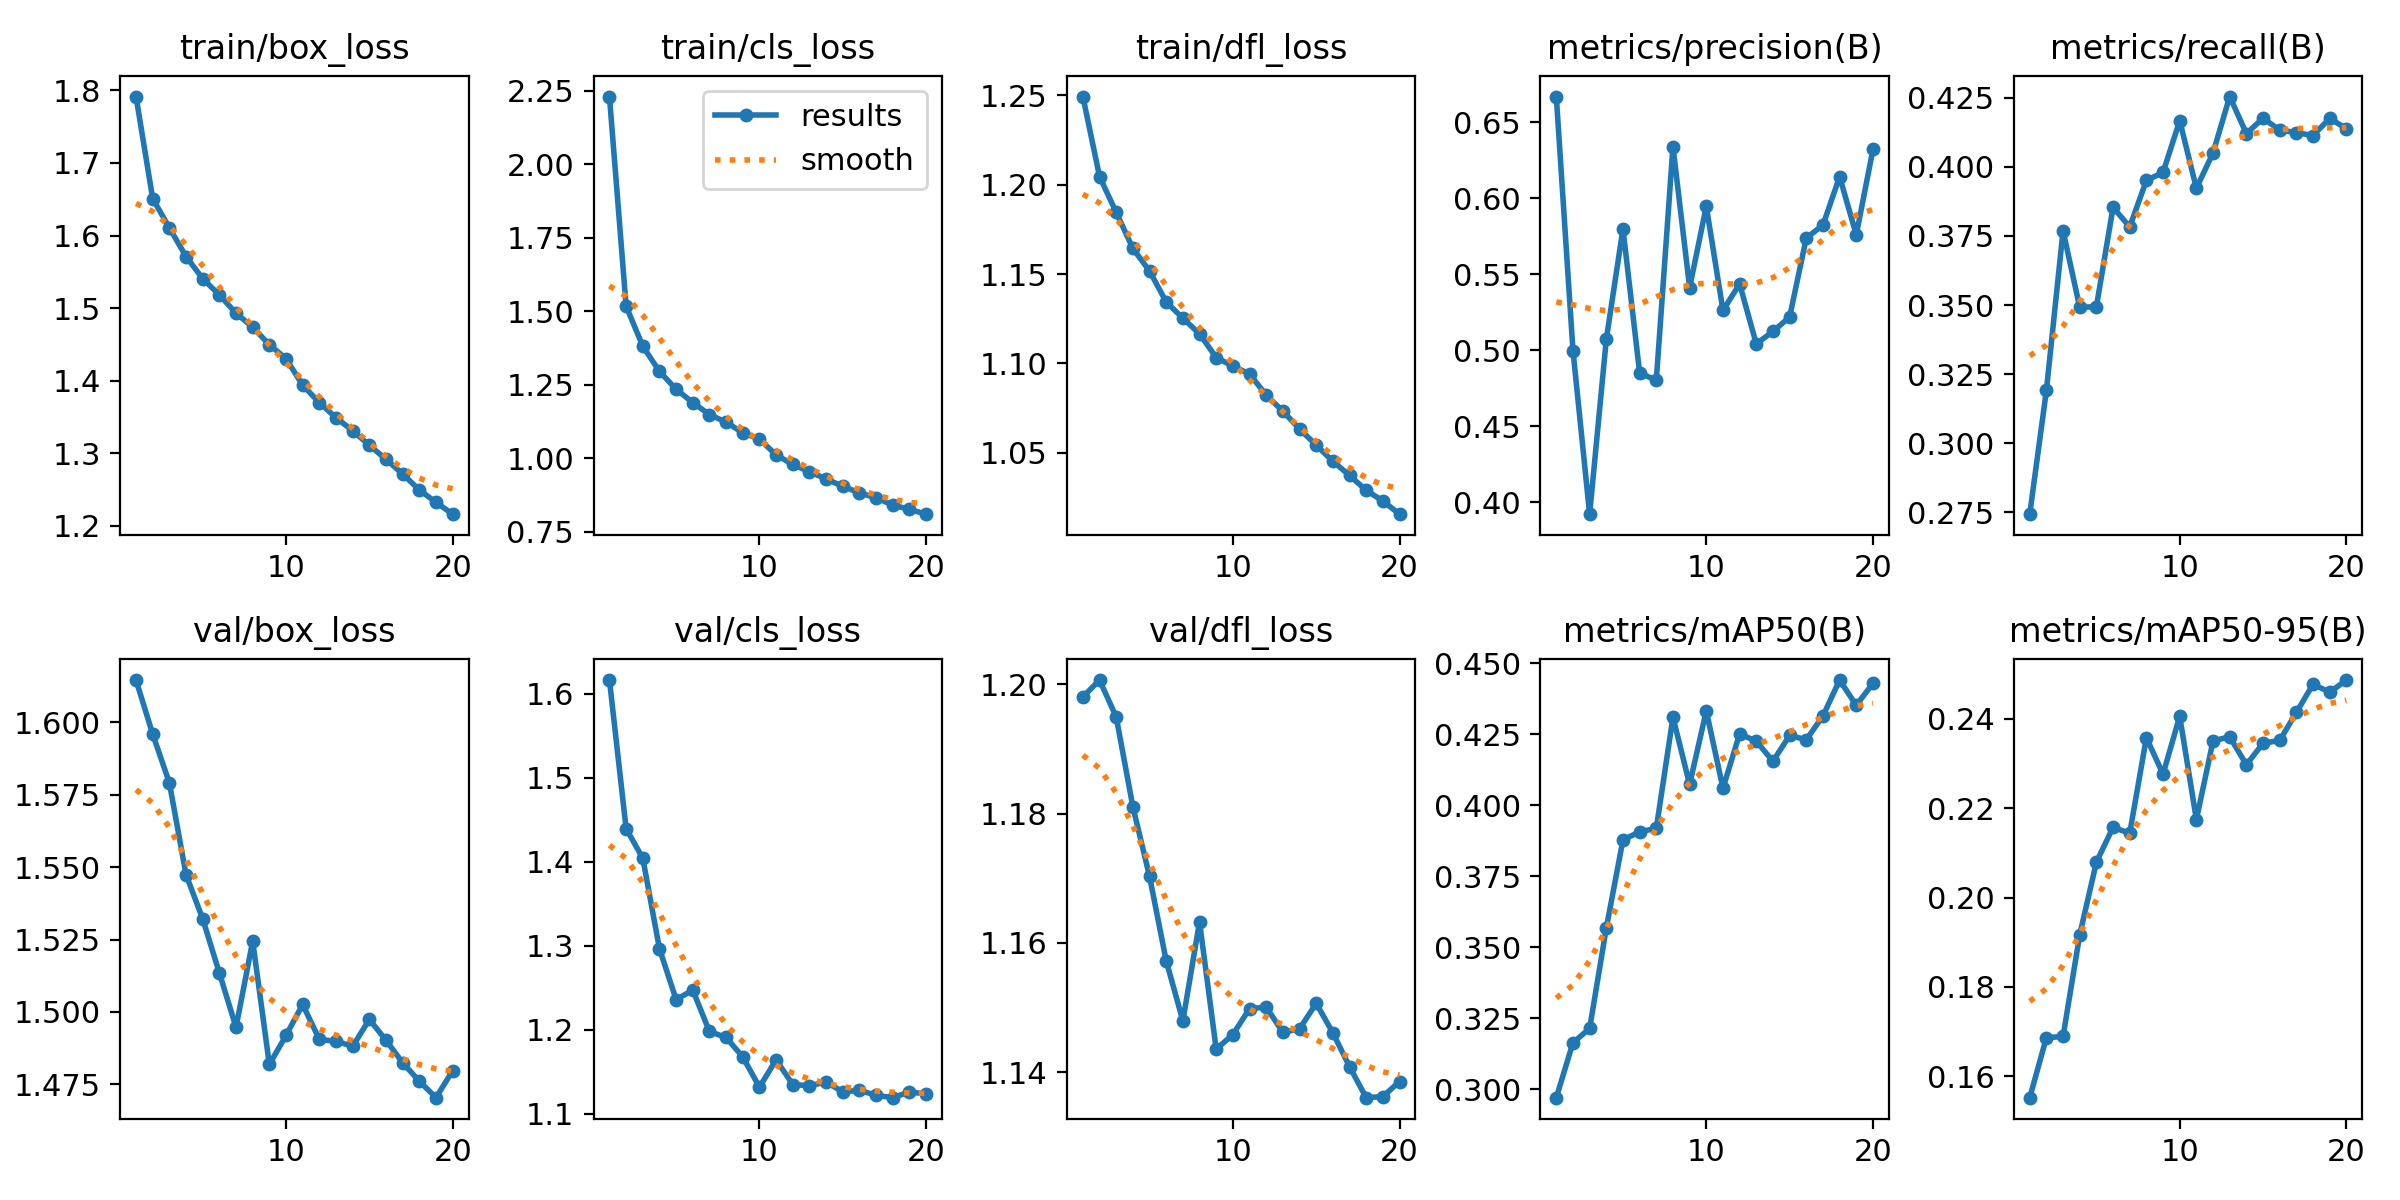
\includegraphics[width=\textwidth]{results.png}
  \caption{20 轮 YOLO11n 训练日志中的损失和验证集曲线。}
  \label{fig:train}
\end{figure}

\subsection{独立 test 集结果与预测核查}

训练结束后，使用验证阶段选出的 \texttt{best.pt}，通过 \texttt{evaluate.py} 显式指定 \texttt{test} 拆分。评估摘要文件只记录 \texttt{test}，对应 2,709 帧独立图像，因此表\ref{tab:test}中的指标是最终检测结果。

\begin{table}[H]
  \centering
  \caption{独立 test 集最终检测指标}
  \label{tab:test}
  \begin{tabular}{lrrrr}
    \toprule
    权重 & Precision & Recall & mAP50 & mAP50--95 \\
    \midrule
    \texttt{best.pt} & 0.511 & 0.394 & 0.403 & 0.217 \\
    \bottomrule
  \end{tabular}
\end{table}

test mAP50 为 0.403，低于训练日志最后一轮 val mAP50 的 0.443；mAP50--95 也从 0.249 降至 0.217。这不是矛盾，而是独立数据对模型泛化的正常检验。因此本报告将 val 曲线用于描述训练趋势，将 test 表用于说明最终性能。

\begin{figure}[H]
  \centering
  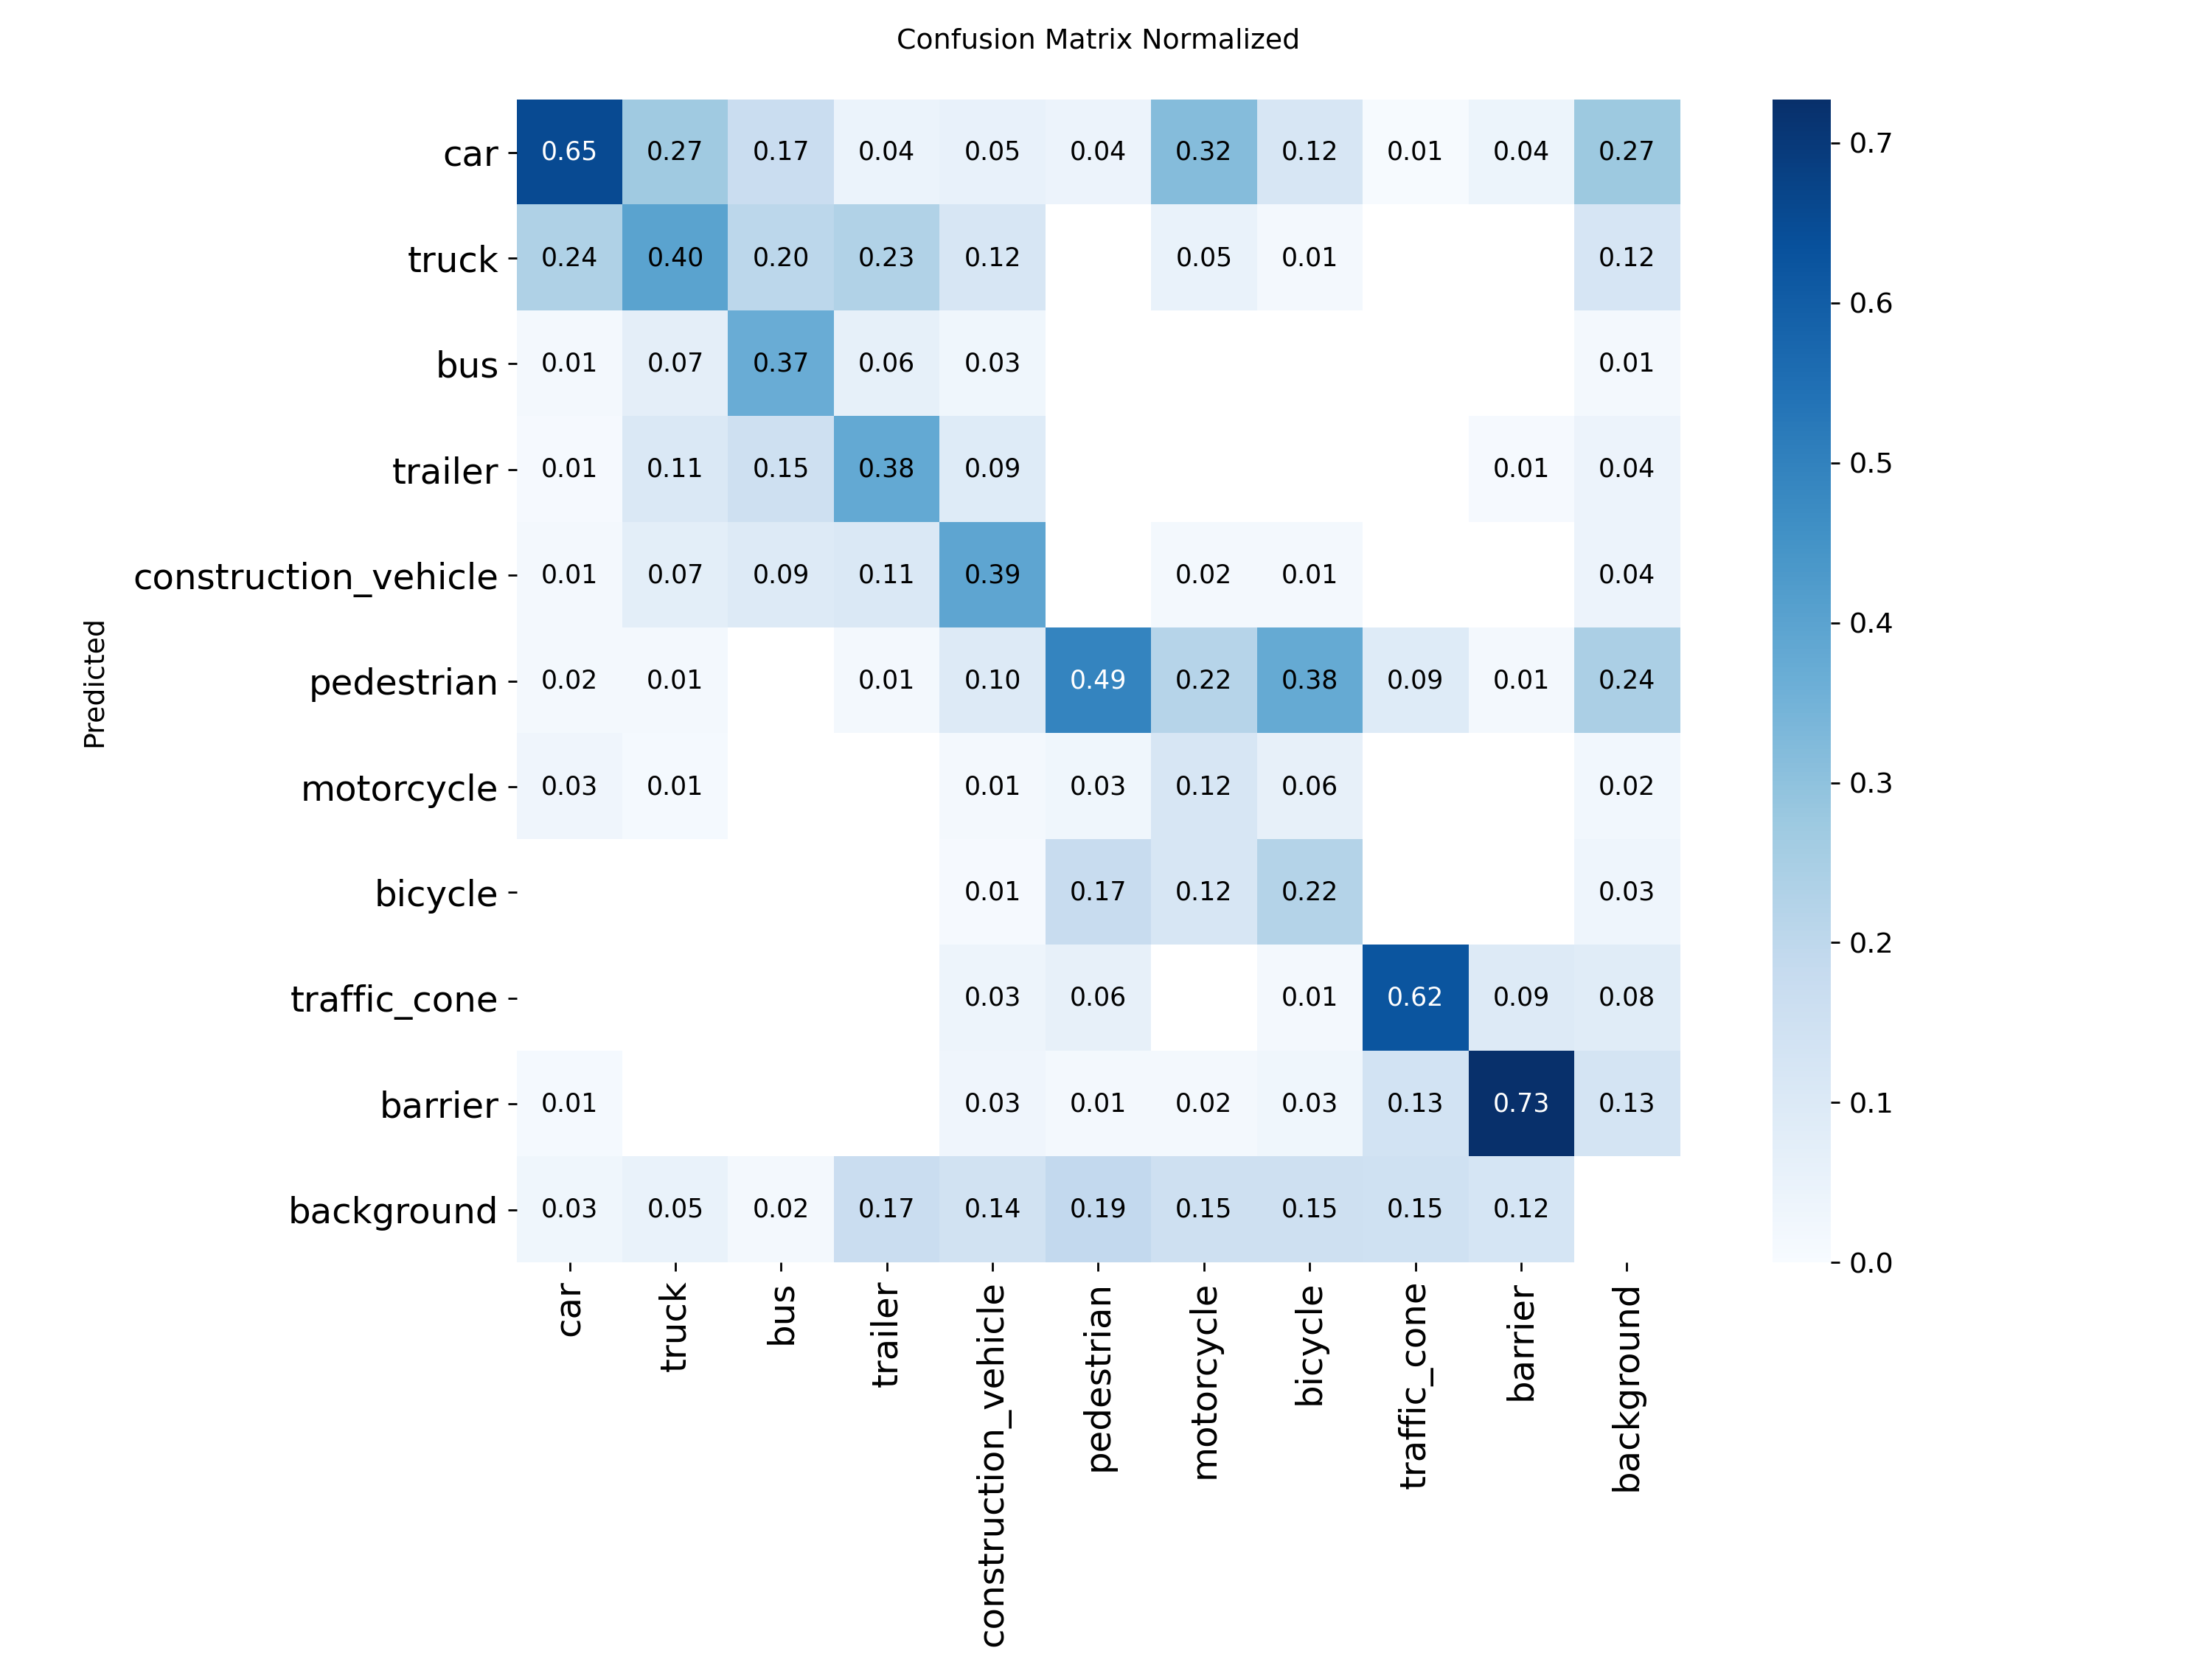
\includegraphics[width=0.82\textwidth,height=0.54\textheight,keepaspectratio]{confusion_matrix_normalized.png}
  \caption{独立 test 集归一化混淆矩阵。}
\end{figure}

\begin{figure}[H]
  \centering
  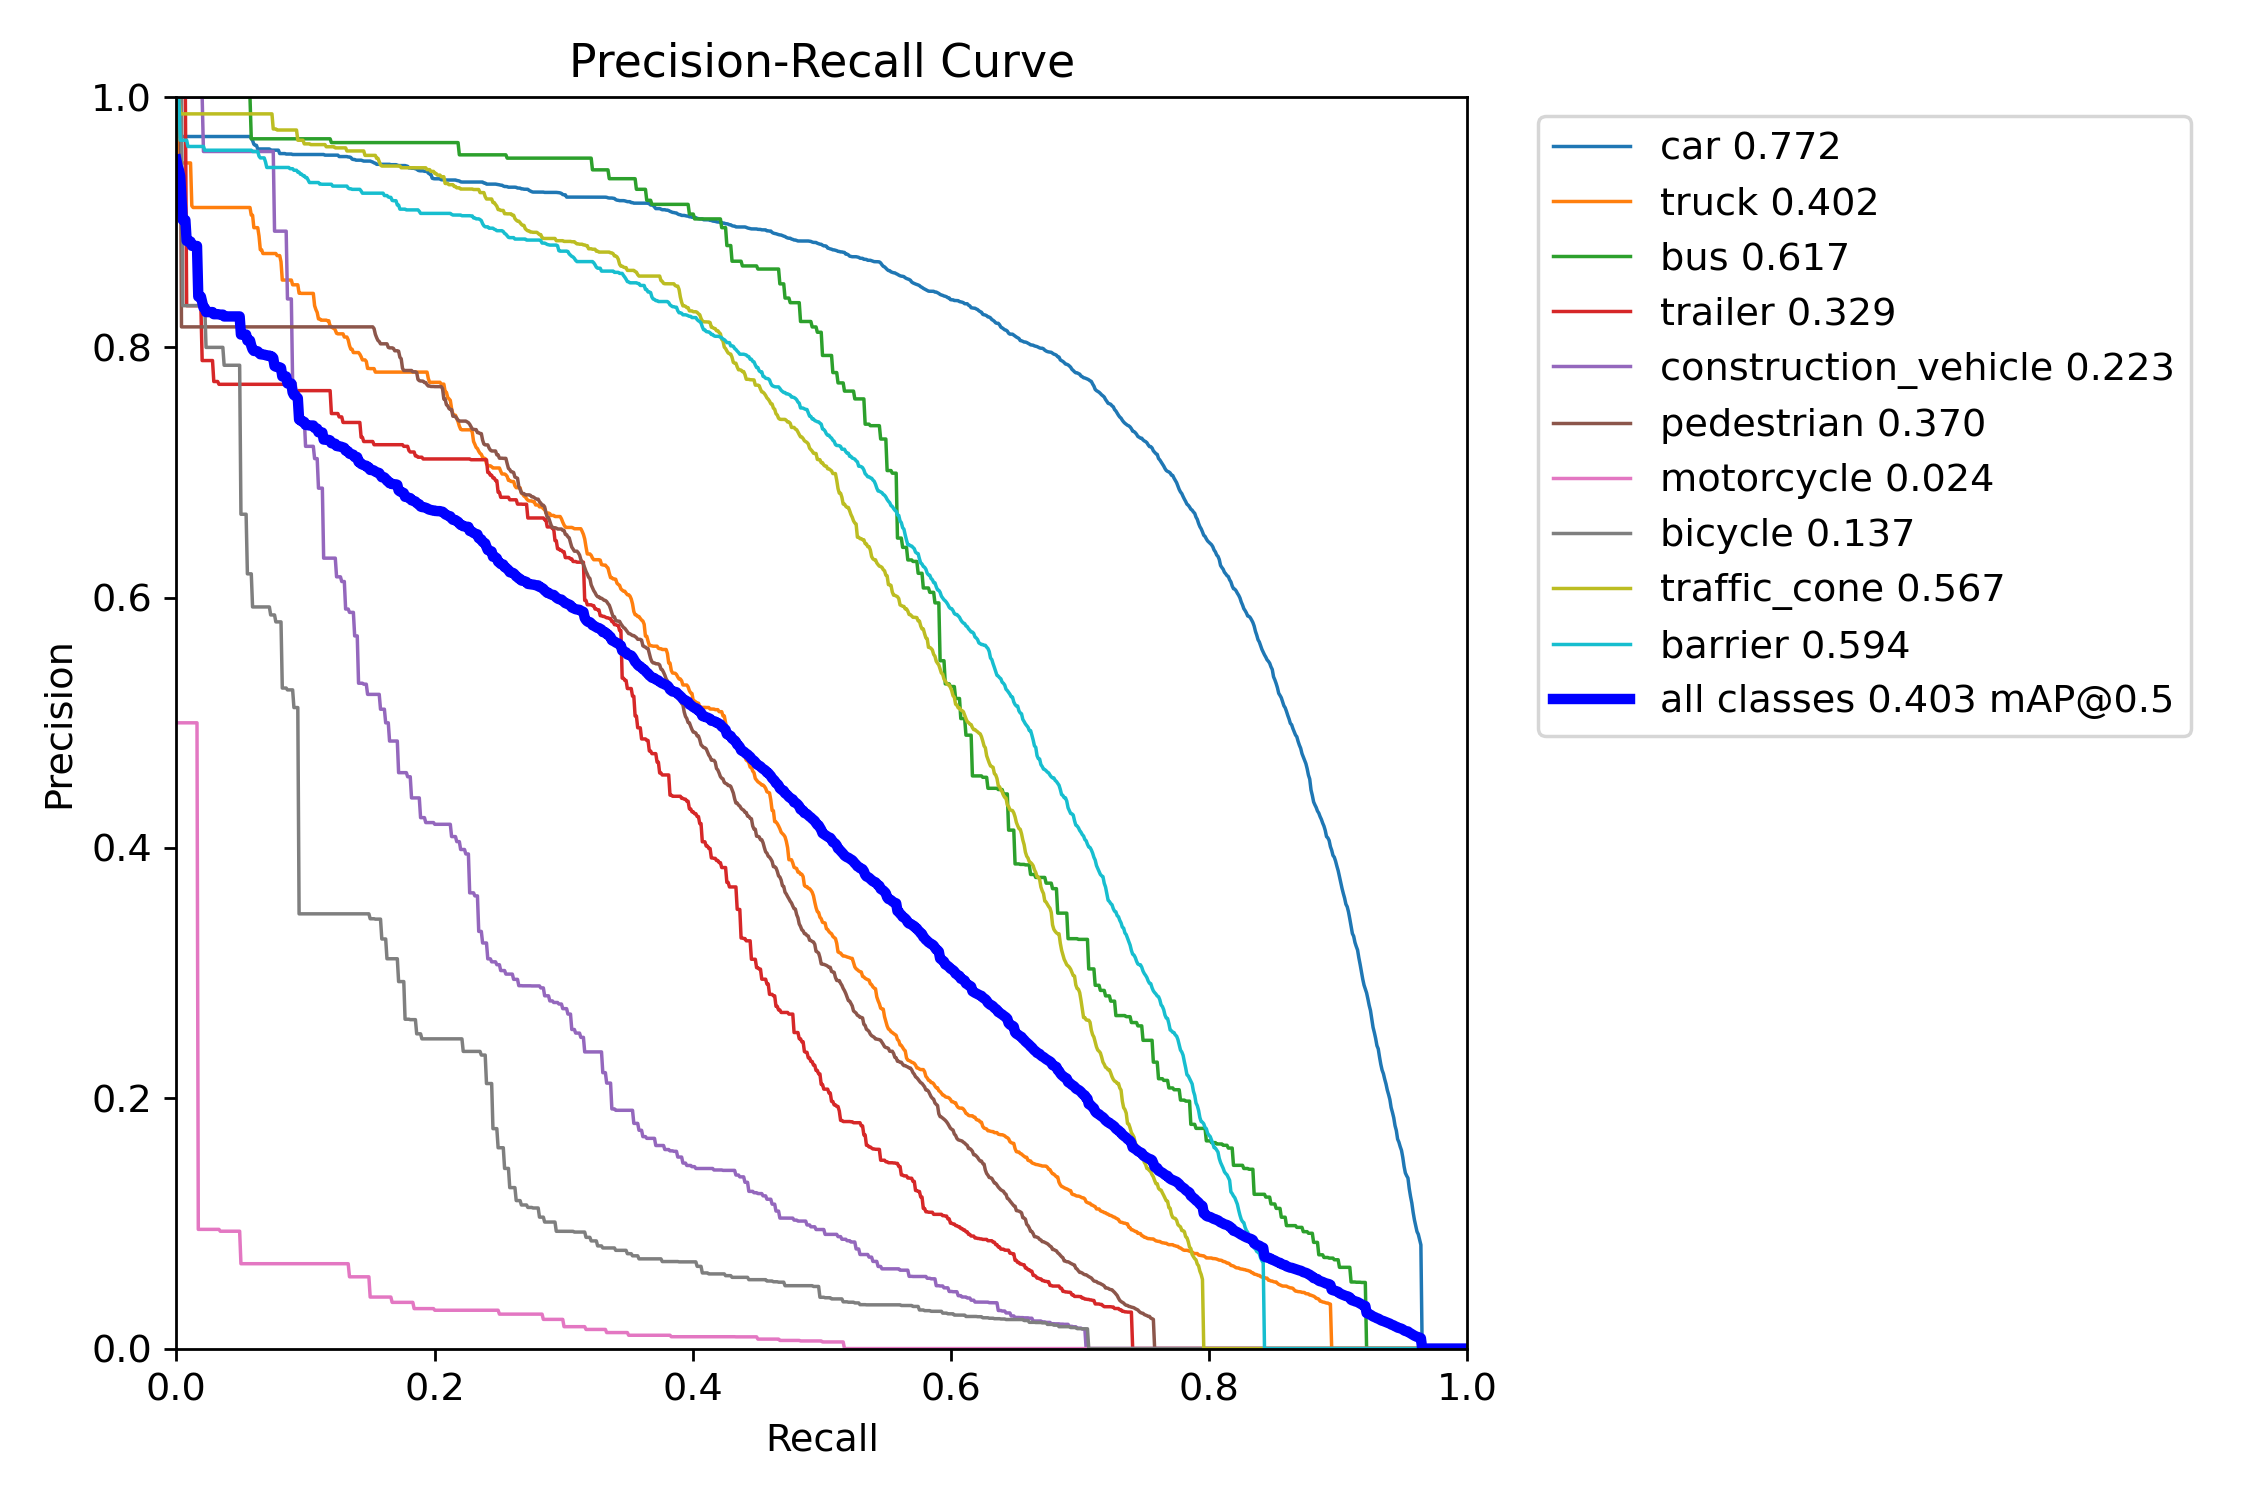
\includegraphics[width=0.48\textwidth]{BoxPR_curve.png}
  \hfill
  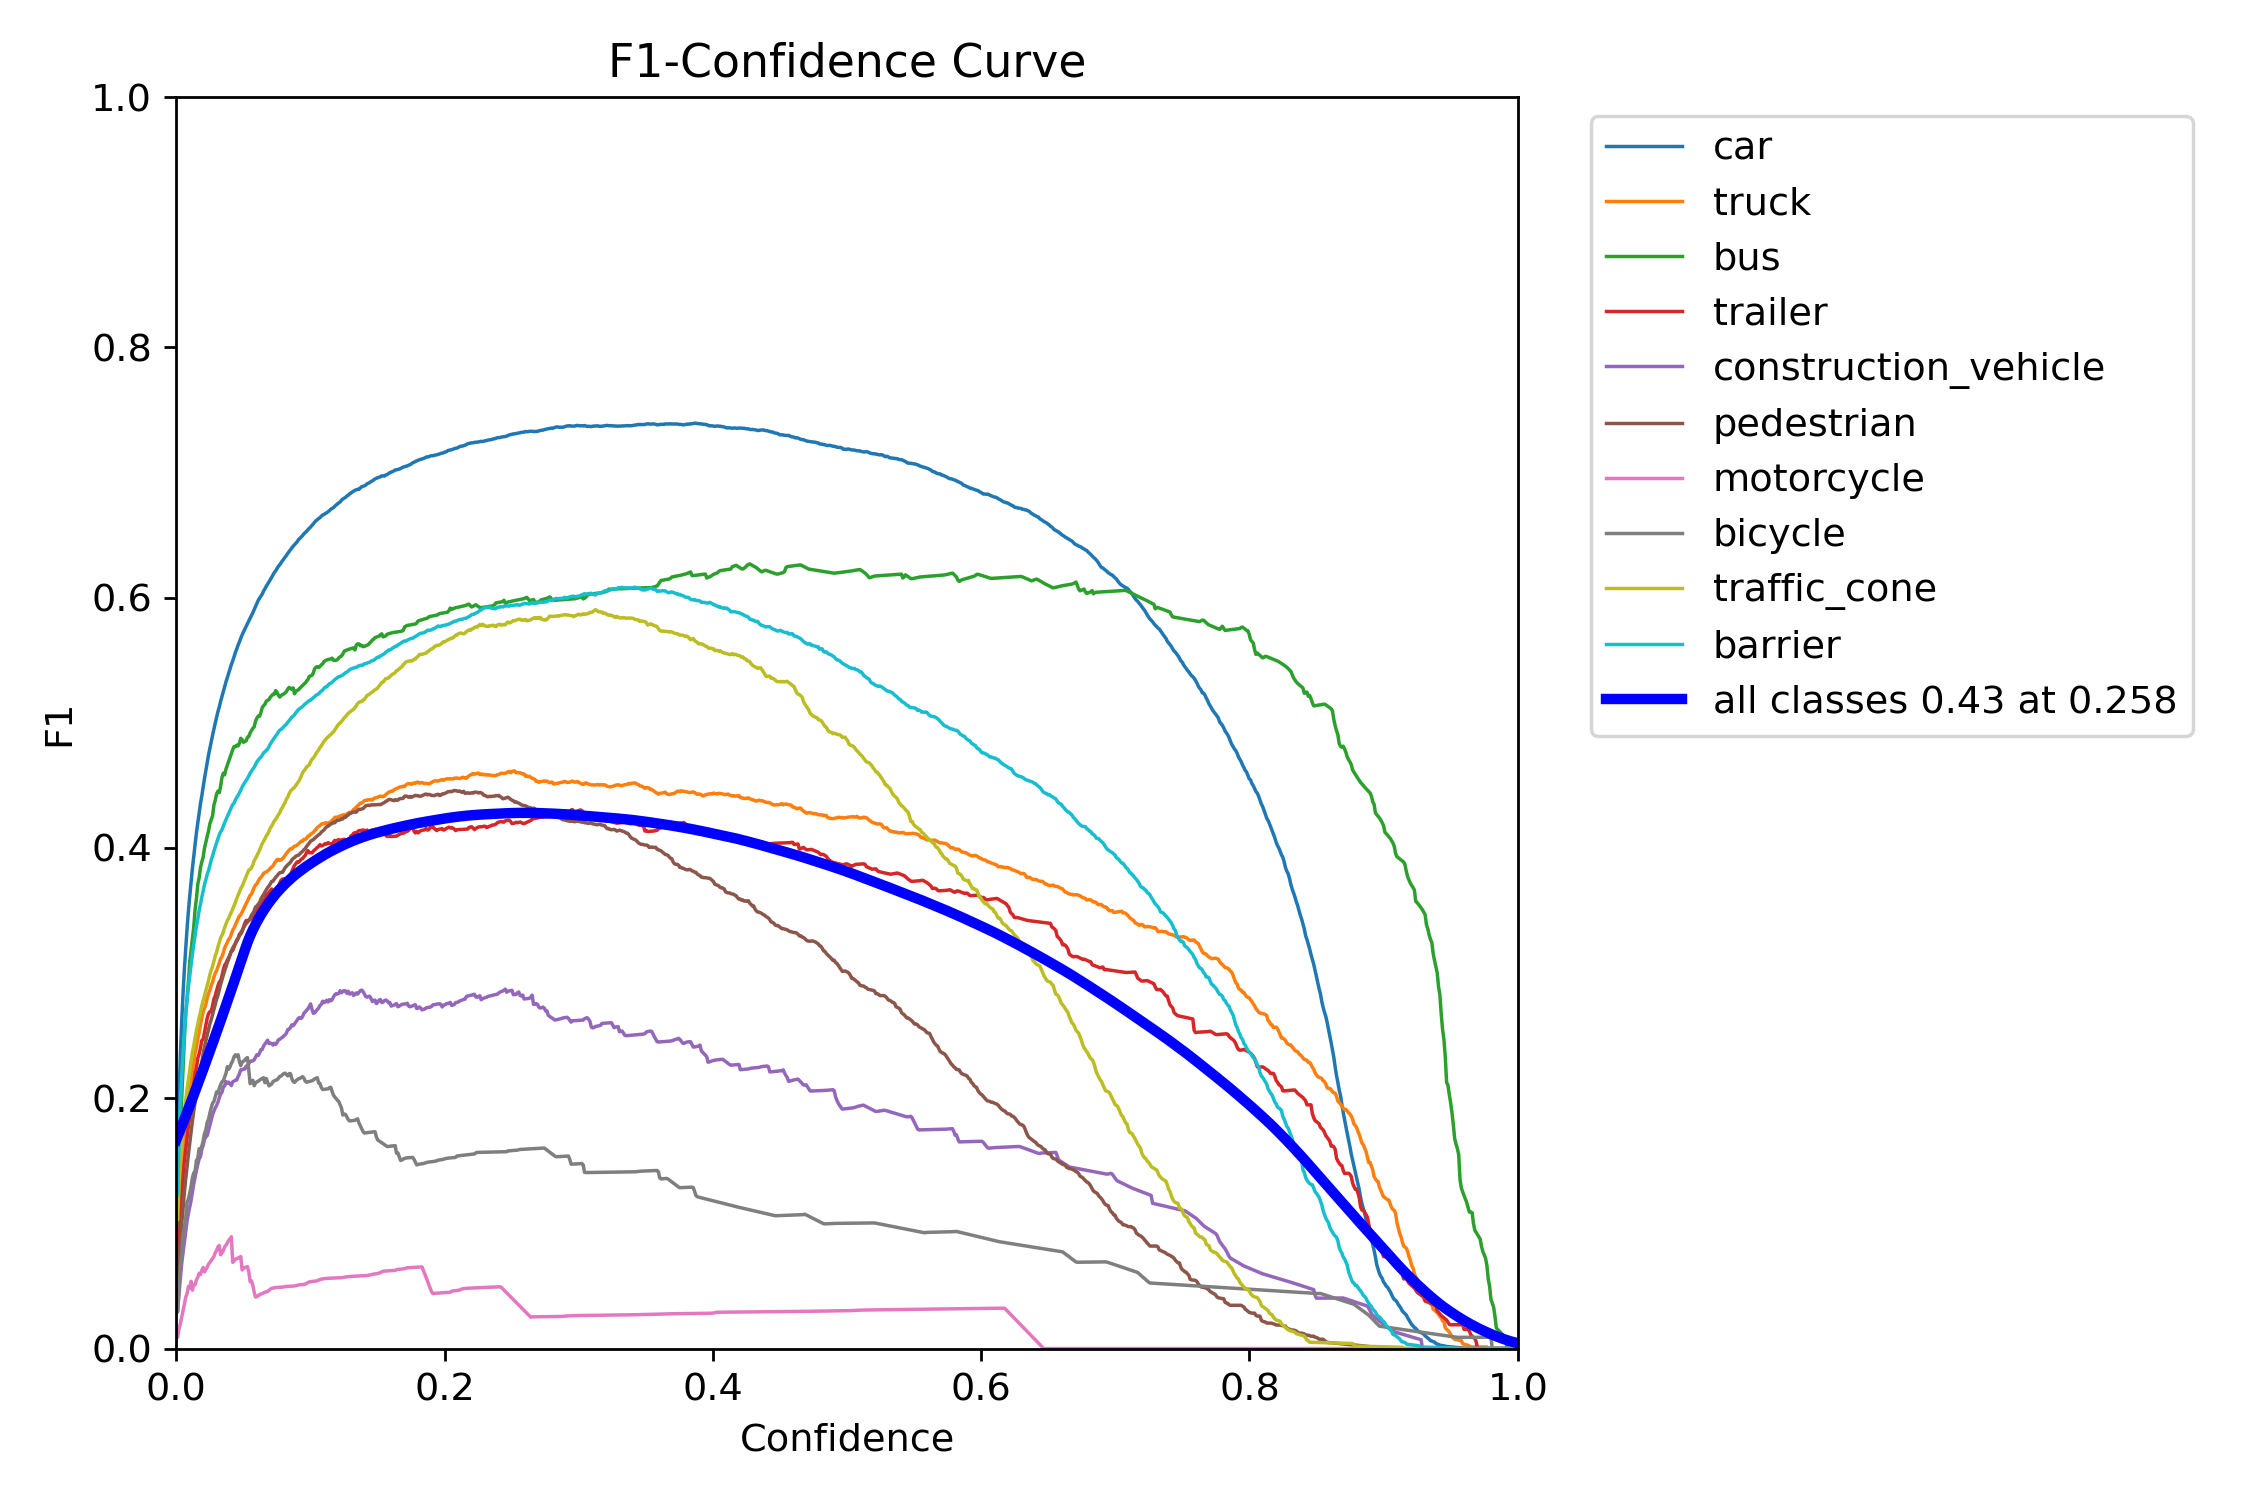
\includegraphics[width=0.48\textwidth]{BoxF1_curve.png}
  \caption{独立 test 集的 PR 曲线（左）和 F1 曲线（右）。}
\end{figure}

\begin{figure}[H]
  \centering
  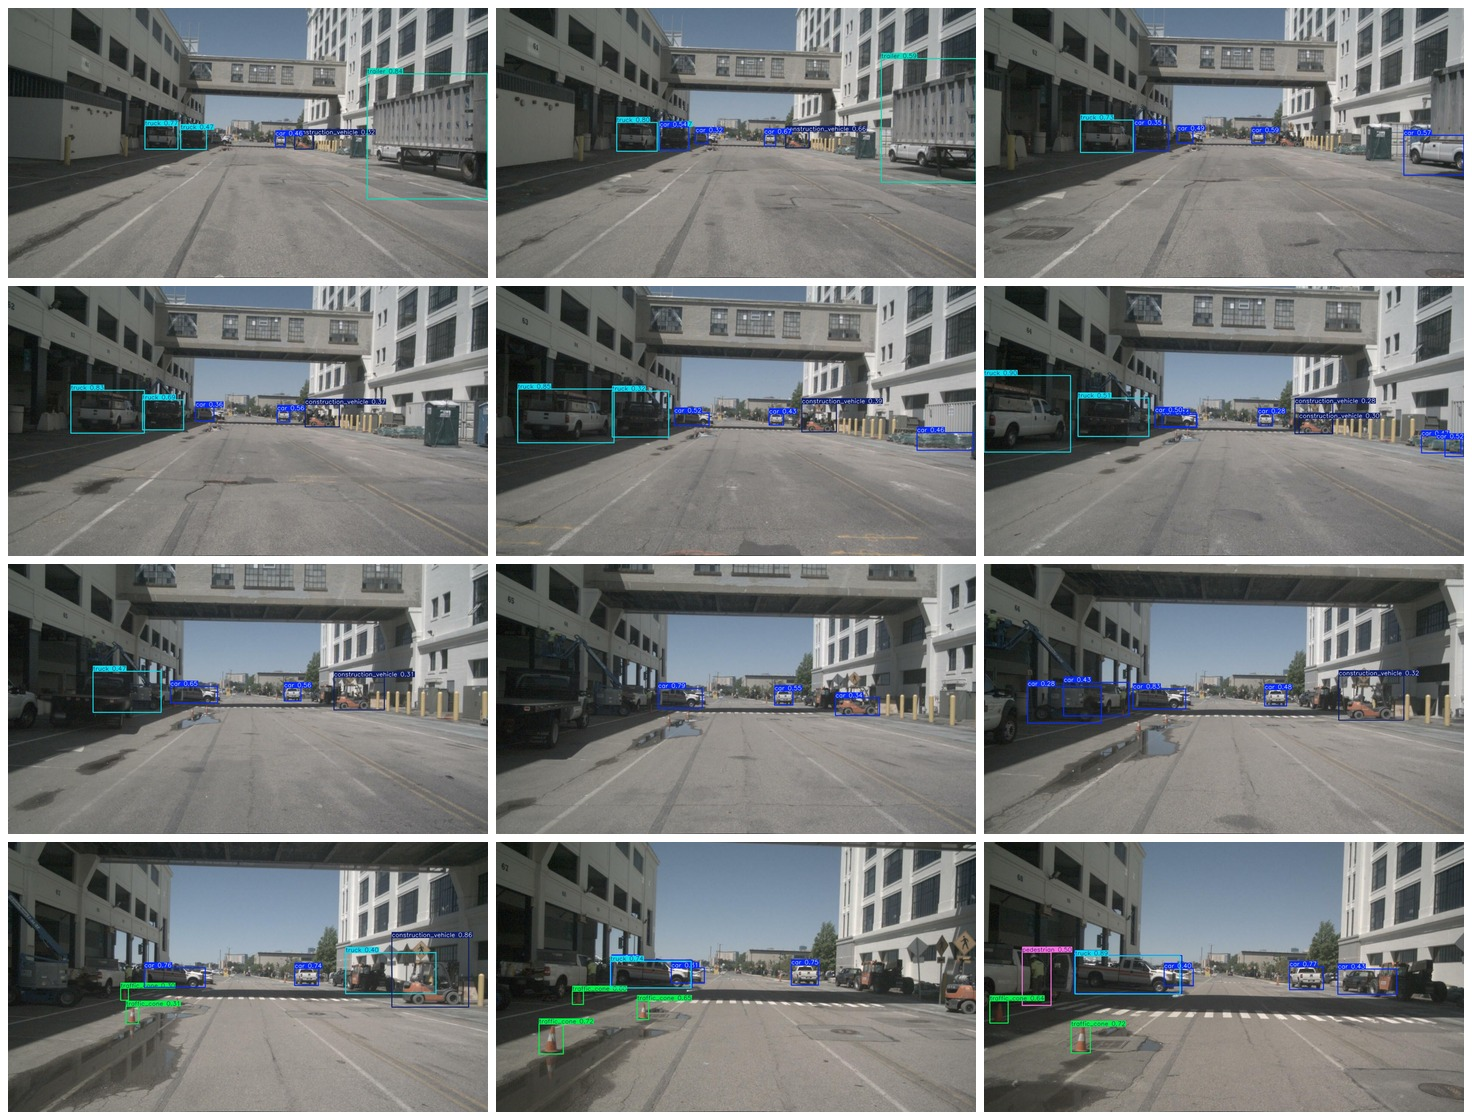
\includegraphics[width=\textwidth]{boston_test_montage.jpg}
  \caption{12 张独立 test 集预测样例。图中为模型输出的类别、置信度和边界框。}
\end{figure}

\section{结论与数据限制}

本实验完成了从 nuScenes 元数据、Camera/LiDAR 感知数据处理到 YOLO 独立测试的完整实践流程。devkit 部分验证了场景、传感器、标定、位姿和 3D 标注之间的连接关系，并在 Boston Seaport 的一个关键帧上实际生成 3D Box 到 2D 图像、LiDAR 俯视图和 LiDAR-相机投影图。YOLO 部分在 20 轮训练后得到独立 test 的 Precision 0.511、Recall 0.394、mAP50 0.403、mAP50--95 0.217。

当前限制来自数据包内容：本地只提供 CAM\_FRONT 与 LIDAR\_TOP 的原始文件，未提供 5 路 Radar 和其余 5 路相机的二进制文件。因此，Radar 的 metadata 访问、点云读取和投影代码已纳入脚本，但没有生成不存在原始数据的 Radar 图。若要补齐真实 Radar 叠加显示，应补充与选定 sample 对应的 Radar PCD 文件后重新运行脚本；不应使用合成点或 LiDAR 点替代 Radar。

\par\smallskip
{\scriptsize\noindent\textbf{依据文件：}nuScenes 元数据 \path{nuscenes/v1.0-trainval/*.json}；可复现 devkit 脚本 \path{scripts/build_devkit_evidence.py} 和输出 \path{output/pdf/assets/devkit/devkit_summary.json}；YOLO 训练记录 \path{yolo_workflow/runs/checkpoints/boston_20ep}；独立评估和预测摘要 \path{yolo_workflow/runs/evaluation/boston_test_summary.json}、\path{yolo_workflow/runs/visualization/boston_test_summary.json}。\par}

\end{document}
